\section{Aspects de la phonétique et de la phonologie du trill, du tap et du flap}

Avant de commencer à décrire les différents segments d'intérêt, nous devons aborder un point terminologique.
Nous avons fait le choix d'utiliser le terme \textsc{trill}. Nous parlerons de \textg{consonne trillée}, et non de \textg{consonne roulée}. Nous mentionnerons la \textg{consonne trill alvéolaire} et la \textg{consonne roulée alvéolaire}. Nous utiliserons le \textg{phonème trill} et non le \textg{phonème roulée}. Ces emprunts à l'anglais, légèrement francisés, se font au dépit de la terminologie francophone pour deux raisons. Premièrement, la plupart de la littérature existante sur les trills est écrite en anglais. La recherche du terme \textg{alveolar trill} dans les ouvrages scientifiques donne lieu à plus de résultats. Deuxièmement, nos travaux s'inscrivent dans une lignée typologique où la terminologie est cruciale pour mettre en contraste les langues et les comparer. Les descriptions des langues sur lesquelles nous nous appuyons mentionnent plus fréquemment le \textg{trill}, ainsi, il nous apparaît naturel de reprendre le terme le plus commun. De même, nous avons sélectionné les termes de \textsc{tap} et de \textsc{flap}, en dépit de la traduction française \textg{consonne battue}.

\begin{figure}
	\centering
	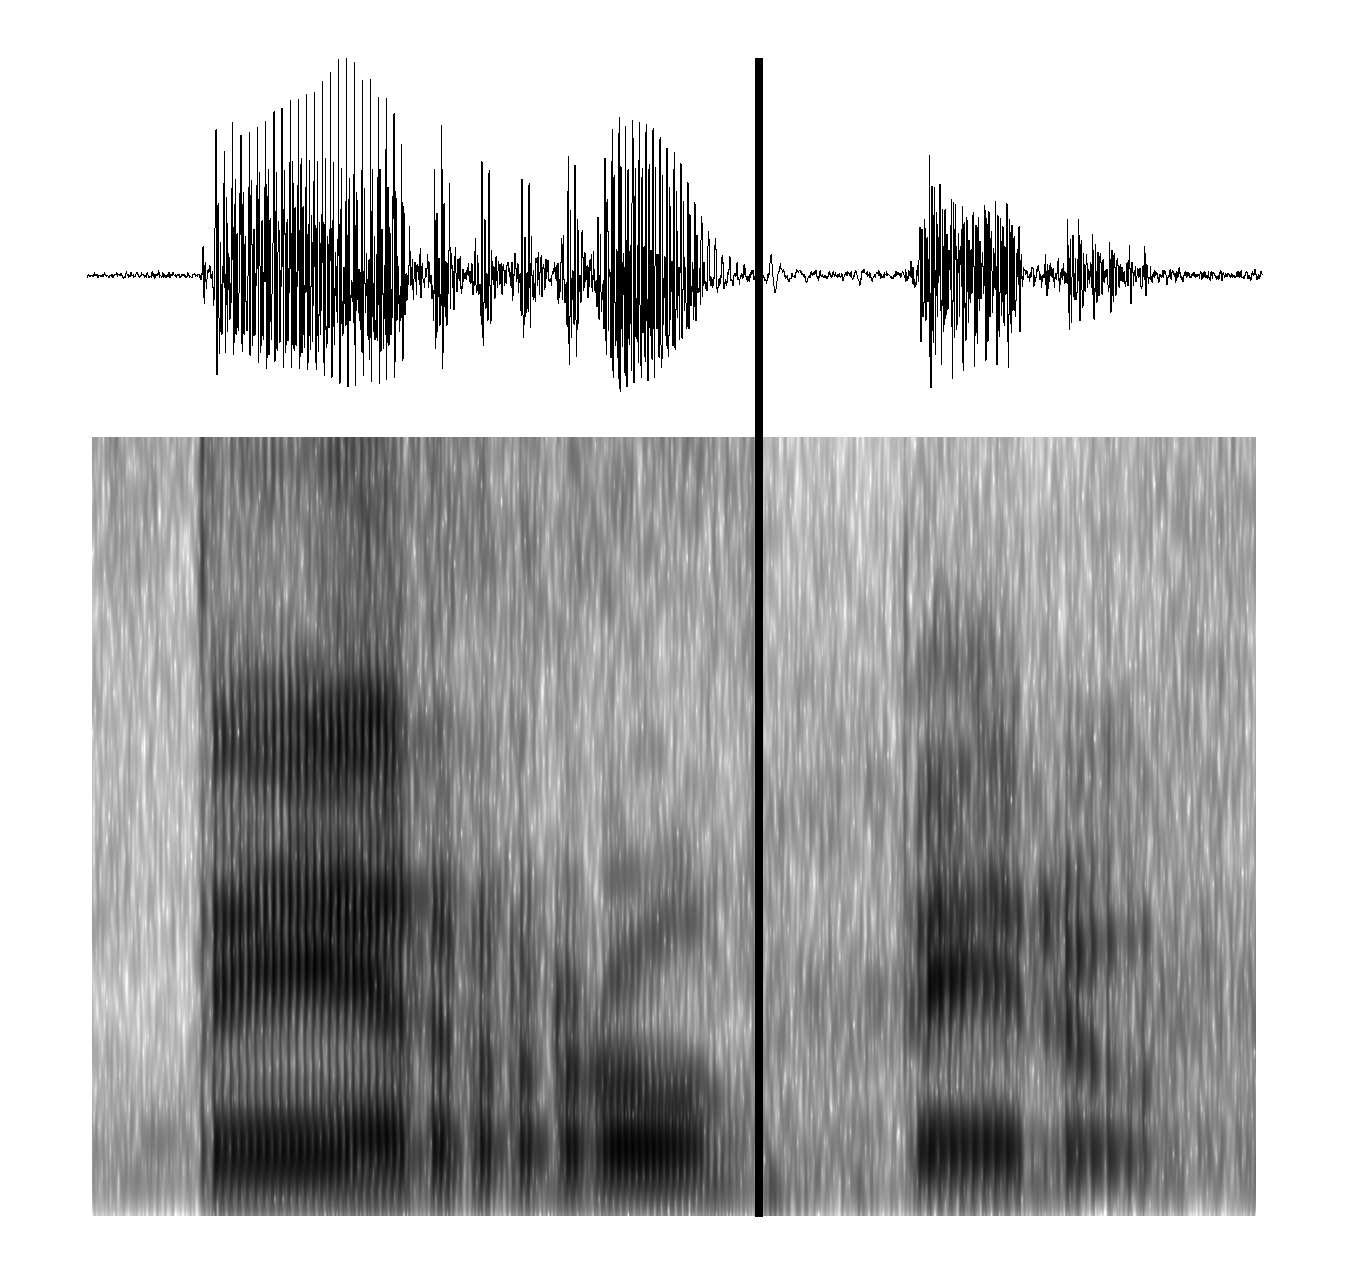
\includegraphics[width=1\linewidth]{rhotiques/images/praat_dogbut.pdf}
	\caption[Illustrations du /r/ et du /ɾ/ en espagnol]{À gauche : le trill dans le mot \textit{perro} /pero/ \textg{chien}. À droite : le tap dans le mot \textit{pero} /ɾ/ \textg{mais}. Les deux exemples sont issus de l'espagnol. Les deux mots ont été produits en isolation, et sont produits par deux locuteurs différents. Le premier (le trill) est produit par un locuteur de 25 ans de Meddelin Antioquia, Colombia, et le second (le tap) par un locuteur de 22 ans de Cartago Valle, Colombia. Le trill et le tap représentés ici sont considérés comme canoniques. L'oscillogramme est donné en haut, et le spectrogramme en bas (les axes sont manquants par choix).}
	\label{fig:praatdogbut}
\end{figure}

\subsection{Description du trill}

Cette sous-section du \textsc{trill} s'intéresse à ce segment d'un point de vue phonétique et phonologique.
Nous reprenons les différentes descriptions de ce segment qui peut impliquer un des trois articulateurs mobiles : les lèvres, la langue, ou l'uvule \parencite{ladefogedLateralsTrills1977}. Il faut souligner que dans cette thèse nous ne nous intéresserons pas aux trills bilabiaux impliquant la vibration des lèvres \parencite{rangelovBilabialTrillsAhamb2019} qui n'ont d'ailleurs jamais été inclus dans la catégorie des rhotiques \parencite{wieseRepresentationRhoticsRepresentation2011}. En ce qui concerne les trills uvulaires, ils sont abordés dans la \autoref{sec:similr} et dans le \autoref{chap:soundcompa}. \\

Nous nous focaliserons uniquement sur la vibration de la pointe de la langue qui donne lieu aux trills apicaux, en laissant de côté celle de la lame de la langue qui donne lieu aux trills laminaux.\\

Contrairement à la sous-section suivante sur le tap/flap, nous ne développerons pas l'origine du terme trill. Cependant, il est important de souligner que le terme peut être ambigu et refléter plusieurs réalités phonétiques de même que le symbole de l'Alphabet Phonétique International \textit{r} (ce point sera développé dans le \autoref{chap:jipa}).

\subsubsection{Acoustique et articulation du trill alvéolaire} \label{subsec:trill}

Le trill alvéolaire apical est un segment produit lorsque la pointe de la langue se maintient de manière lâche près de la crête alvéolaire, de sorte qu'un mouvement d'air fasse vibrer la pointe de la langue. Cela se traduit par des périodes où la langue touche la crête puis s'en sépare \parencite[318]{ladefogedCoursePhonetics2015}.
\textcite[49]{ladefogedLateralsTrills1977} suggèrent que peu de langues possèdent des trills, et que les trills de ces langues sont généralement alvéolaires. Les trills réalisés avec la pointe de la langue ont une fréquence de vibration moyenne de 28,6Hz $\pm$ 4,0.\footnote{\textcite{ladefogedLateralsTrills1977} trouvent que les trills produits avec d'autres articulateurs ont aussi une fréquence de vibration similaire ce qui peut expliquer un degré de similarité auditoire.} \textcite{lindauStory1985} obtient une fréquence de 25Hz sur son échantillon multilingue (soit 1 cycle toutes les 40ms) avec généralement deux à trois périodes. Le nombre de périodes dépend de différents facteurs
\footnote{Certains des facteurs sont développés en \autoref{subsec:trill_tap}.} qui peuvent être linguistiques (le contexte phonologique, la position dans le mot, l'accentuation de la syllabe, le nombre de syllabes du mot, la catégorie grammaticale) \parencite[cf. tableau p. 23 pour les études d'intérêt]{zahlerVariationistAccountTrill2014} et non-linguistiques (le sexe, l'âge [notons que les effets de l'âge et du sexe ne sont pas les mêmes en fonction des études], la classe sociale, le lieu de vie, les croyances, la densité du réseau social des locuteurs, ou encore le style de tâche effectuée pour la récolte de données) \parencite[cf. tableau p. 21-22 pour les études d'intérêt]{zahlerVariationistAccountTrill2014}.\\

Ainsi le trill est souvent caractérisé par la présence d'au moins deux périodes visibles au niveau du signal acoustique (\autoref{fig:praatdogbut}). Chaque période est composée d'une phase de contact (similaire à une obstruction; nous emploierons le terme de \textg{contact} ou d'\textg{obstruction} dans la suite de cette thèse) et une période de relâchement. Le trill à une période reste néanmoins possible, son articulation étant différente du tap/flap \parencite{spajicTrillsToda1996}.

\begin{displayquote}
	\textrm{[...]} even in cases where there is only a single contact with the roof of the mouth, the action is physiologically (but perhaps not auditorily) quite distinct from that of a tap. \parencite[p.50]{ladefogedPreliminariesLinguisticPhonetics1971}
\end{displayquote}


De plus, le trill est caractérisé par des prérequis aérodynamiques fins. \textcite{soleAerodynamicCharacteristicsTrills2002} cherche des tendances universelles dans le comportement des trills. L'autrice montre qu'en cas de manquement des pré-requis aérodynamiques, le segment ne sera pas trillé et/ou dévoisé (le tap est différent de nature et n'a pas de tels prérequis cf. \autoref{subsec:acous_tap_flap}).
En outre, \textcite{mcgowanTongueTipTrills1992} montre que la position de la langue, sa forme et son élasticité, ainsi qu'une différence de pression de part et d'autre de la constriction de la pointe de la langue, jouent un rôle dans l'initiation de la vibration.
\textcite{dhananjayaAcousticAnalysisTrill2012} suggèrent que triller entraîne une géométrie du tract oral qui change rapidement, ce qui rend les trills moins directs à étudier.
Ce sont les différents prérequis du trill qui en font un segment complexe et un des derniers acquis dans les langues du monde \parencite{mcleodChildrenConsonantAcquisition2018}.\\

Il n'existe pas à notre connaissance d'autres études sur la perception du trill, et de la discrimination de contraste de longueur, au sein d'une même langue autre que celle de \textcite{raymondInitialMedialGeminate2005}. Cette étude sur l'arop-lopek \glotto{arop1243}, langue parlée en Papouasie-Nouvelle-Guinée par quelques 3000 locuteurs/trices, s'intéresse au contraste entre le /r/ et le /rr/, la contrepartie géminée du /r/. Le flap [ɾ] est aussi présent dans la langue comme allophone intervocalique du /d/.
Trois études sont incluses dans l'article.
La première étude se focalise sur la production des trills et s'intéresse au nombre minimum, moyen et maximum de contacts que les trills et les trills géminées peuvent avoir.
La deuxième étude cherche à savoir si les locuteurs sont capables de discriminer, faire la différence entre un trill géminé et un trill non géminé. 
Finalement, la dernière étude se concentre sur la compréhension de la frontière de perception entre un trill et un trill géminé.\\

\textcite{raymondInitialMedialGeminate2005} ont enregistré six locuteurs mâles pour leur étude de production lors d'une tâche de lecture de liste de mots. Les trills en position intervocalique et finale pouvaient avoir au minimum un contact (88/364) ce qui n'était pas le cas lorsqu'ils étaient en position initiale (0/131). Certains trills géminés étaient aussi produits avec un contact, bien que ce n'était pas les productions les plus fréquentes (5 occurrences sur 218). Les trills en position initiale sont plus longs que les trills dans les autres positions.
Les trills ont été produits avec maximum 5 contacts, alors que les trills géminés ont été produits avec maximum 7 contacts.
Les trills géminés sont produits avec plus de contacts (en moyenne 3,76 contacts) que les trills non géminés (en moyenne 2,29 contacts).
L'étude de discrimination sur le terrain a permis de mettre en avant que les locuteurs sont capables de discriminer correctement un trill d'un trill géminé en position initiale et intervocalique. L'étude de perception sert à montrer qu'à partir de trills modifiés artificiellement, les locuteurs catégorisent dans les trills, les items avec moins de contacts, et dans les trills géminés, ceux avec le plus de contacts. De même que pour l'étude en production, une asymétrie existe entre les items en position initiale et ceux en position intervocalique. En position initiale, il faut plus de contacts pour qu'un item soit considéré comme un trill géminé.\\

La position en début de mot est favorable aux trills. Cependant, les rhotiques ont tendance a être défavorisées en initiale de mot à travers les langues \parencite{labruneWordinitialRhoticAvoidance2021}. Ces résultats sont néanmoins à mettre en contraste avec \textcite{kavitskayaTrillsPalatalizationConsequences2009} qui, sur la base de données du russe, montrent que le trill est défavorisé en position intervocalique. Cela permettrait d'expliquer les distributions des différents allophones des rhotiques cross-linguistiquement.\\


Les trills sont souvent étudiés par rapport à des langues indo-européennes, à l'exception de quelques études typologiques.
L'étude de \textcite{raymondInitialMedialGeminate2005} est intéressante car elle apporte de la phonologie de laboratoire sur le terrain avec une expérience de production, de discrimination et de perception. De plus, elle s'intéresse à une langue sous-étudiée (sur \href{https://www.google.com/maps/place/Matafum,+Papouasie-Nouvelle-Guin\%C3\%A9e/@-5.2182111,146.4002482,9.13z/data=!4m13!1m7!3m6!1s0x68f3e3520a551b3f:0x58a83294038393a4!2sLong+Island!3b1!8m2!3d-5.3535839!4d147.1464245!3m4!1s0x68f3fd93309894d3:0x2df33848a2f3c3c0!8m2!3d-5.3707325!4d147.0343745}{Long Island} en Papouasie-Nouvelle-Guinée) dans une aire géographique et dans une famille linguistique (austronésienne) et permet d'apporter des éléments de réflexion sur le contraste que peuvent faire les langues entre trois sons \textg{simil-r} : le flap, le trill et le trill géminé.


\subsection{Description du tap et du flap}

Après avoir décrit les principales caractéristiques du trill, nous décrivons le tap et le flap. Nous avons pris le soin de développer cette sous-section sur le tap et le flap car \textg{
[t]he alveolar tap is a fairly understudied rhotic, and many aspects of its variation within and between speakers as well as across languages are not fully known \parencite[86]{cathcartArticulatoryVariationAlveolar2012}}. Tout d'abord nous aborderons l'historique des termes tap et flap avant de décrire articulatoirement et acoustiquement ces segments.

\subsubsection{Terminologie et historique du tap/flap}

\begin{figure}
	\centering
	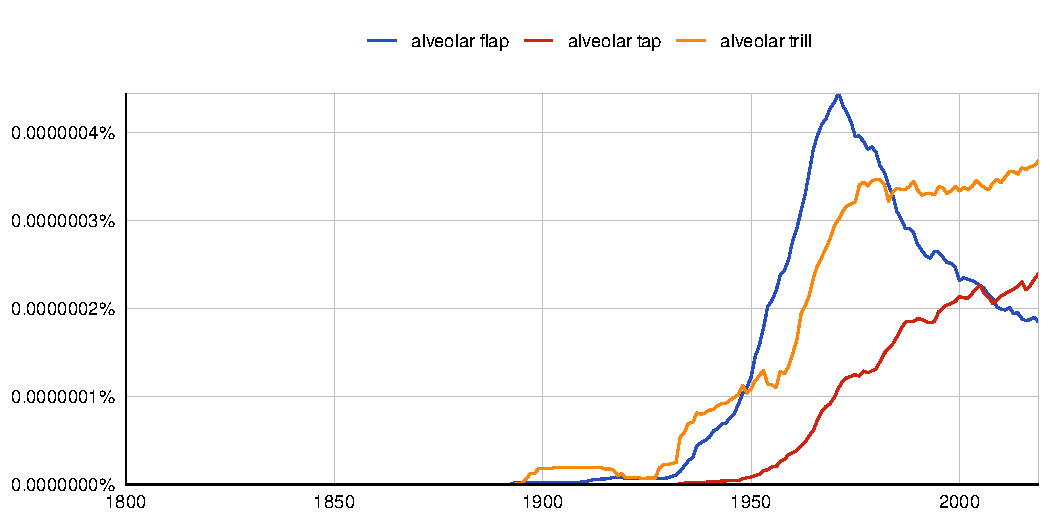
\includegraphics[width=1\linewidth]{images/google_ngram_trill_tap_flap}
	\caption[Google n-grams de \textg{alveolar trill}, \textg{alveolar tap}, \textg{alveolar flap}]{Fréquence des expressions \textg{alveolar trill}, \textg{alveolar tap}, \textg{alveolar flap} à partir des données de Google Books en utilisant le package \texttt{ngramr} sur \texttt{RStudio} \parencite{rcoreteamLanguageEnvironmentStatistical2020}, à partir du jeu de données de Google 2019.}
	\label{fig:googlengramtrilltapflap}
\end{figure}


On retrouve deux grandes approches concernant les taps et flaps. D'un côté, les études qui s'intéressent aux segments en prenant comme langue de référence l'anglais parlé aux États-Unis où le [ɾ] est un allophones des obstruentes /t, d/. De l'autre côté, il s'agit des études qui opposent le tap et le flap au trill car dans les langues étudiées on retrouve deux phonèmes /ɾ/ et /r/ comme en catalan. Il existe aussi une littérature moins abondante qui s'intéresse aux taps et flaps avec un point de vue utilisant d'autres langues.\\

Le \textg{trill} est apparu en premier, suivi du \textg{flap} puis du \textg{tap}. De la même manière, le symbole \textit{r} est apparu avant le \textit{ɾ} dans l'Alphabet Phonétique International. Nous avons fait le choix de garder le terme tap dans cette thèse comme terme générique pour parler des taps et des flaps. Nous justifions ce choix par l'éducation linguistique que nous avons reçue où le terme \textg{tap} était plus fréquent que le terme \textg{flap} reflétant leurs usages dans les publications scientifiques (Figure \ref{fig:googlengramtrilltapflap}). Le terme de flap est vraisemblablement d'abord apparu sur le continent européen où on le retrouve rapidement dans les publications de \textit{Le maître phonétique}. L'espagnol y était décrit avec un flap \parencite[8]{passySupplementAimPrincipales1904} et un trill. Le terme de tap, lui, est sûrement apparu sur le continent américain pour faire spécifiquement référence à l'allophone battu du /t/ et du /d/ produit en anglais américain entre deux voyelles. On retrouve dès les années 40 avec John Samuel Kenyon et Kenneth L. Pike l'apparition du terme \textg{tap}.

\begin{displayquote}
Voiced \textbf{t} is often described as a single-tap \textbf{r}. To the author's ear the two are quite distinct. Even when the voiced \textbf{t} has repeated taps (trilled  \textbf{t}) it is acoustically distinct from trilled \textbf{r} [...] \parencite[127]{kenyonAmericanPronunciation1943}
\end{displayquote}


\begin{displayquote}
In \textit{flap articulation} the articulator gives one rapid tap against its articulating region and then immediately releases; approach and release together are formed by a single ballistic movement. \parencite[124-125]{pikePhoneticsCriticalAnalysis1943}\
\end{displayquote}

En 1964, \citeauthor{ladefogedPhoneticStudyWest1968}\footnote{Nous n'avons pu consulter que la version de 1968.} publie un ouvrage sur les langues d'Afrique de l'ouest dans lequel il met en évidence que le hausa \glotto{haus1257} contraste entre un tap, qui peut être réalisé comme un trill, et un flap. Il s'agit de la première occurrence que nous avons trouvée où le tap est explicitement opposé au flap. Ses travaux lui permettront en \citeyear{ladefogedPreliminariesLinguisticPhonetics1971} de définir le tap comme un son où \textg{[o]ne articulator [is] thrown against another} et le flap comme un son où \textg{[o]ne articulator striking another one is passing} \parencite[46]{ladefogedPreliminariesLinguisticPhonetics1971}. Ces descriptions vont évoluer au fil des recherches menées sur les deux sons avec une influence sur le reste de la linguistique descriptive de terrain (comme nous le verrons avec les différences de terminologie dans le \autoref{chap:metagram}).

\begin{displayquote}
Alveolar tap ɾ also occurs in Hausa. Most of my informants used this sound, although occasionally it was replaced by a trilled r. Both these sounds occurred where Hausa orthography has r. There is also a contrasting sound which is sometimes written as r, and which appears to be a retroflex flap ɽ. [...] The nearest I can come to agreeing with this is to say that the first sound is a trill which has a statistical probability of consisting of only one tap. \parencite[30]{ladefogedPhoneticStudyWest1968}
\end{displayquote}

Cette section a servi à mettre en évidence que l'existence des deux termes tap et flap est historiquement justifiée. Les publications contemporaines font souvent le choix d'un terme ou de l'autre (ce qui n'est pas problématique, cela n'ayant pas de conséquences pour les analyses).\footnote{Par exemple, dans notre \autoref{chap:jipa} sur les \textit{Illustrations of the IPA} nous avait fait le choix (qui n'était pas vraiment éclairé au moment de l'écriture) d'utiliser le terme \textg{tap}.}

\subsection{Acoustique et articulation du tap/flap} \label{subsec:acous_tap_flap}

Nous détaillons dans cette sous-partie les différentes études qui ont eu comme objet de recherche le tap et/ou le flap.
\textcite[128]{catfordFundamentalProblemsPhonetics1977}, se basant sur les travaux de \textcite{ladefogedPhoneticStudyWest1968}, utilise le terme \textg{flap}. Le flap est articulatoirement décrit comme un son produit lorsqu'un organe articulatoire approche un autre (stationnaire) créant un contact momentané avant de se retirer (aussi connu sous le nom de \textg{one-tap r}). Deux types de flaps sont mis en avant en fonction de la mise en action de la langue. D'un côté, les flaps \textg{flick} [ɾ] sont produits lorsque l'articulateur revient à sa position de départ, et de l'autre, les flaps \textg{transient} [ɽ] sont produits lorsque l'articulateur mobile entre en contact momentané avec l'articulateur fixe dans son mouvement vers une position finale (Figure \ref{fig:figure29catford}). Les deux types de segments ont une durée comprise entre 10 et 30ms.\\

\begin{figure}
	\centering
	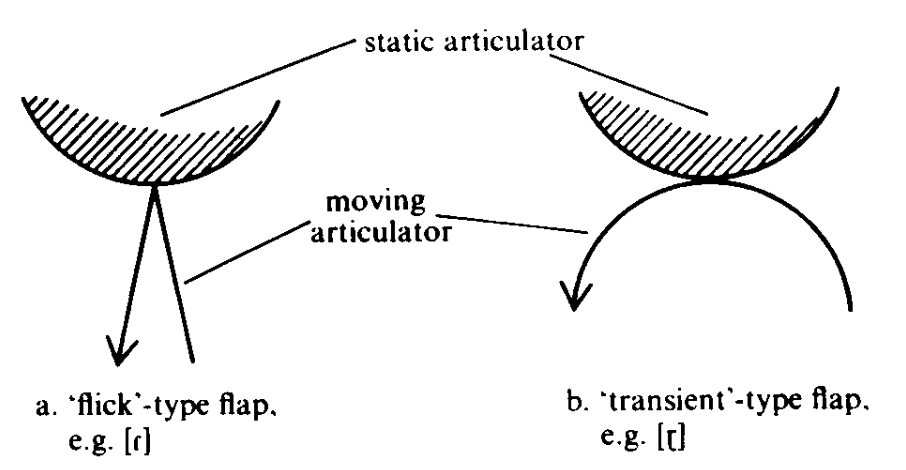
\includegraphics[width=0.9\linewidth]{rhotiques/images/figure_29_catford}
	\caption[Schématisation des \textg{flaps}. Figure issue de Catford (1977)]{Schématisation par \textcite[129]{catfordFundamentalProblemsPhonetics1977} des deux types de flaps identifiés. L'un sera généralement repris par la littérature comme un tap [ɾ], et l'autre comme un flap [ɽ].}
	\label{fig:figure29catford}
\end{figure}

\textcite[129]{catfordFundamentalProblemsPhonetics1977} souligne l'importance de la momentanéité des flaps, des mouvements balistiques, les opposant aux stops : \textg{a stop can be prolonged; a flap cannot be prolonged}.\footnote{\textcite[397]{newmanHausaLanguageEncyclopedic2000} mentionne qu'en hausa le flap géminé existe de même que le \textg{tap/roll} geminé. Le flap géminé se manifeste phonétiquement par une augmentation de la \textg{temporal period of the retroflex flap gesture}, là où le \textg{tap/roll} devient un trill discernable. \textcite[237]{ladefogedSoundsWorldLanguages1996}, en hausa, analysent la géminée du flap comme une longue approximante rétroflexe.} Contrairement aux stops, les flaps mettent en jeu une surface de contact moins importante selon \textcite[251]{catfordFundamentalProblemsPhonetics1977}.\\

En anglais américain, le flap peut être un allophone du /t/ et du /d/. Le flap est un des allophones des occlusives alvéolaires en position post-voyelle accentuée \parencite{zueAcousticStudyMedial1979}.
Avec des enregistrements de trois hommes et trois femmes, les auteurs analysent les données et soulignent la présence de variation dans les réalisations des flaps. En effet, la phase de \textg{closure} peut être plus ou moins complète. Lorsqu'elle est partielle, on peut retrouver au niveau du signal acoustique de la turbulence similaire à celle qu'on peut retrouver avec les fricatives voisées. Les auteurs mesurent en moyenne 27 ms pour les /d/ et 26 ms pour les /t/ avec un écart autour de la moyenne entre 10 ms et 40 ms, principalement dû au contexte vocalique. Une durée courte de flap indique un mouvement rapide de la langue montant et descendant de la pointe de la langue, alors qu'une durée longue est indicatrice d'une pression accumulée pendant la constriction de la langue qui s'accompagne d'un relâchement accompagné par une explosion de bruit visible sur le spectrogramme. Cela peut s'expliquer par la position du corps de la langue. S'il est bas, alors le mouvement de la pointe de la langue peut être bref, alors que s'il est haut, le mouvement de la pointe de la langue \textg{overshoot} la zone alvéolaire rendant l'occlusion plus longue.\\


\textcite{zengUnderstandingFlappingXiangxiang2007} s'intéresse aux flaps dans le dialecte chinois de Xiangxiang\footnote{Selon nous, il est regrettable que cette description allophonique ne soit pas présente dans l'\textit{Illustration of the IPA} publiée, disponible en FirstView (cf. \autoref{subsec:data_coll}) à propos du même dialecte du chinois \parencite{zengXiangxiangDialectChinese2020}. Nous nous interrogeons donc sur la proportion des langues décrites dans JIPA à avoir des occlusives qui sont réalisées comme des flaps dans certains contextes, mais qui ne sont pas décrites comme telles.} qui sont des allophones du /d/ et du /t$^\textrm{\tiny h}$/ en position intervocalique pré-syllabe accentuée et pré-syllabe non accentuée. L'étude se base sur quatre locuteurs et une locutrice et permet de mettre en évidence de la variation intra-individuelle. \citeauthor{zengUnderstandingFlappingXiangxiang2007} montre qu'il existe dans cette position pour le /d/ un continuum allant du [d] \textg{typique}, avec une occlusion longue et une barre d'explosion, au flap, avec une occlusion de courte durée et sans barre d'explosion. Dans ce continuum, on retrouve aussi le flap long avec une durée plus longue que le flap typique, et le [d] court avec une durée d'occlusion plus courte que celle du [d] typique.
Un dernier variant, considéré comme \textg{extrême} par \citeauthor{zengUnderstandingFlappingXiangxiang2007}, possède une structure similaire à celle d'une approximante, c'est-à-dire avec un degré moindre de constriction orale. Pour le /t$^\textrm{\tiny h}$/, cinq variants sont identifiés :

\begin{itemize}
\item le typique [t$^\textrm{\tiny h}$],
\item le typique [d$^\textrm{\tiny h}$],
\item le court [d$^\textrm{\tiny h}$],
\item le flap aspiré long
\item et le flap aspiré typique.
\end{itemize} 

Des données aérodynamiques sont aussi incluses et permettent de montrer une relation entre le flux d'air oral et les différents motifs acoustiques.
Ainsi, \textcite{zengUnderstandingFlappingXiangxiang2007} montre que le processus de \textg{flapping} n'est pas binaire. L'accentuation de la voyelle précédente est exclue comme facteur explicatif des différents variants mais les voyelles précédentes et suivantes permettent d'expliquer la variation à cause de co-articulation.\\

\textcite{sonPitfallsSpectrogramReadings2008}, dans la continuité de \textcite{zengUnderstandingFlappingXiangxiang2007}, s'intéresse au flap allophone de la liquide /l/ en coréen. Son étude inclut des données acoustiques de deux locutrices native de Séoul en plus de mesures articulométriques. \citeauthor{sonPitfallsSpectrogramReadings2008} met en évidence de la variation intra-individuelle avec cinq variants :

\begin{itemize}
	\item Flap voisé avec explosion
	\item Flap voisé sans explosion
	\item Flap partiellement voisé avec explosion
	\item Flap non voisé avec explosion
	\item Flap \textg{extrême} (reprenant la description de \textcite{zengUnderstandingFlappingXiangxiang2007})
\end{itemize}

L'étude articulatoire a permis de montrer que, même lorsqu'il n'y avait pas de constriction dans le cas des flaps extrêmes, il y avait quand même un mouvement large de la pointe de la langue, mettant en évidence une certaine invariance dans l'articulation du flap. Cette invariance est donc à mettre en contraste avec la variation dans les résultats des études acoustiques.\\

Les travaux initiés par Derrick, Gick et leurs collègues \parencite{derrickQuantitativeAnalysisSubphonemic2008,derrickTwoPhonologicalSegments2010,derrickIndividualVariationEnglish2011,derrickAcousticCorrelatesFlaps2013} sur la base d'ultrasons ont permis de mettre en avant la variation dans les mouvement associés au processus de \textg{flapping} en anglais américain. On retrouve quatre variants (Figure \ref{fig:tapflap}):

\begin{itemize}
	\item Up-flap
	\item Down-flap
	\item Alveolar tap - le tap alvéolaire
	\item Postalveolar tap - le tap post-alvéolaire
\end{itemize} 

La catégorisation des différents variants s'est faite en fonction du mouvement de la pointe de la langue, ainsi que de sa direction. Les travaux préliminaires de \textcite{derrickQuantitativeAnalysisSubphonemic2008} montrent que tous les participants produisent les quatre variants et que la variation est influencée par la position de la langue avant et après le segment \parencite{derrickTwoPhonologicalSegments2010}. \textcite{derrickIndividualVariationEnglish2011}, en étudiant huit locutrices et dix locuteurs, obtiennent que trois participants n'ont pas produit un des variants (le tap post-alvéolaire). Ainsi, les auteurs montrent que les réalisations \textg{flap} sont plus fréquentes que les réalisations \textg{tap}. On retrouve en plus de la variation non-conditionnée puisque pour les mêmes mots, certains participants ont utilisé différentes stratégies articulatoires. \\

\begin{figure}
	\centering
	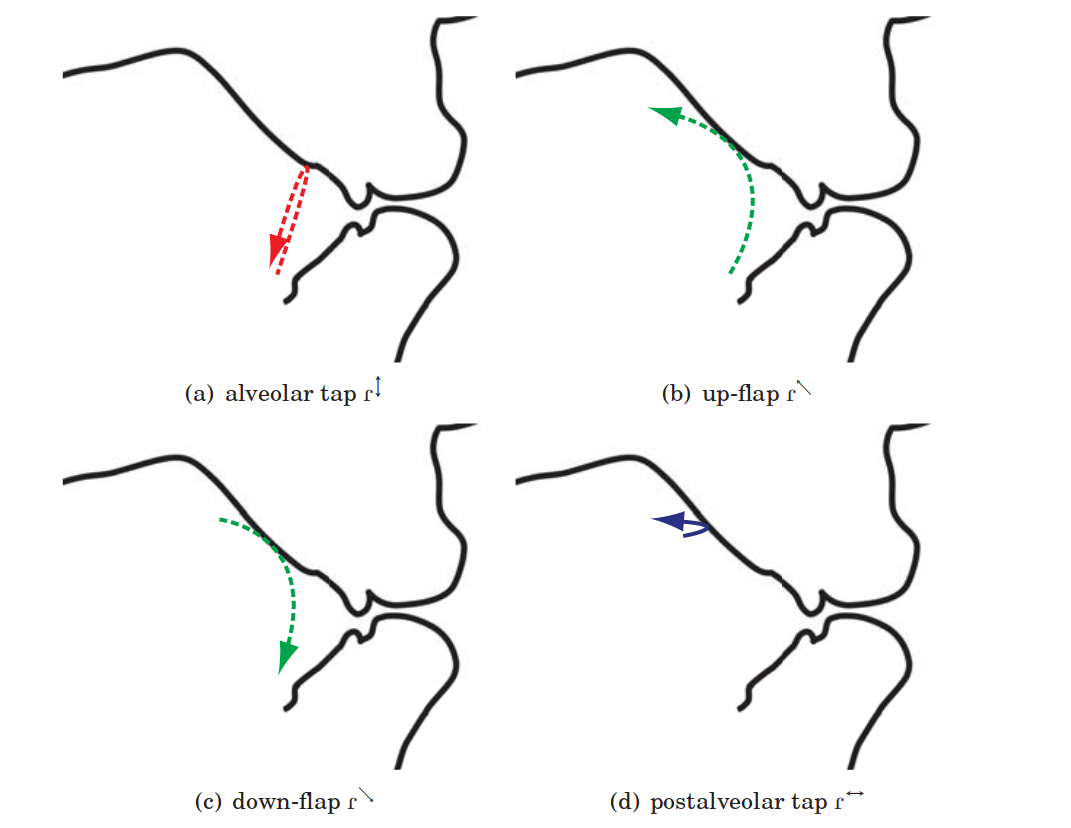
\includegraphics[width=0.7\linewidth]{rhotiques/images/tap_flap}
	\caption[Différents mouvements pour le tap/flap en anglais américain. Figure issue de \textcite{derrickAcousticCorrelatesFlaps2013}]{Les différents mouvements pour le tap/flap en anglais américain. La figure est issue de \textcite{derrickAcousticCorrelatesFlaps2013}. Les différents mouvements ont été obtenus par ultrason.}
	\label{fig:tapflap}
\end{figure}

\textcite{derrickIndividualVariationEnglish2011} offrent un nouveau regard sur les données de différentes langues. Pour eux, les contrastes entre les quatre différents variants du flap sont possibles. Ils mettent en avant des contrastes phonétiques sur la base de contrastes entre tap et flap, comme c'est le cas pour le punjabi\footnote{Il existe une \textit{Illustration of the IPA} pour le punjabi \parencite{hussainPunjabiLyallpuriVariety2019} où les auteurs mentionnent un contraste entre deux rhotiques : un tap alvéolaire /ɾ/ et un tap rétroflexe /ɽ/ (\textg{retroflex tap} [\textit{sic}] (p. 6). Les auteurs illustrent une paire minimale et explicitent que la consonne rétroflexe met en avant un abaissement précoce des troisième et quatrième formants.} \parencite[645]{shacklePanjabi2003}, ou le norvégien où l'on retrouve un [ɾ] s'opposant à un [ɽ] dans certains dialectes \parencite[24]{kristoffersenPhonologyNorwegian2000}.\\

L'étude préliminaire de 2013 de \citeauthor{derrickAcousticCorrelatesFlaps2013} s'intéresse à l'acoustique des quatre variants. Les auteurs montrent qu'il y a des différences significatives pour la fréquence fondamentale et les cinq premiers formants entre les variants. Des deux premiers formants, les auteurs concluent que les quatre variants ont des configurations différentes en termes d'aperture et de postériorité, mais que ces différences se réduisent après la consonne. En ce qui concerne le troisième formant, les auteurs concluent que les variants ont différents points de contact. Le down flap a son point de contact le plus proche des dents, suivi du tap alvéolaire et du up flap, et c'est le tap post-alvéolaire qui a son point de contact le plus haut.\\

Dans certains cas, le tap/flap n'est pas considéré comme un allophone d'un stop mais d'une rhotique, c'est le cas de l'espagnol ou du catalan où le tap a été étudié en opposition à une autre rhotique de ces langues : le trill. Nous avons détaillé les études sur le trill en \autoref{subsec:trill} et nous faisons le lien entre les deux segments en \autoref{subsec:trill_tap}. Dans cette section, nous ne parlerons que du tap/flap.

\textcite{recasensProductionCharacteristicsApicoalveolar1991} étudie de manière préliminaire les caractéristiques de production du tap apico-alvéolaire en catalan avec l'électropalatographie sur la base de ses propres productions.
L'occlusion n'est pas systématiquement complète pour le tap. Il y a plus de contact pour le tap lorsqu'il est précédé et suivi par une voyelle postérieure [a, u] que lorsqu'il est précédé et suivi par une voyelle antérieure [i]. Ce manque de contact associé à la voyelle antérieure [i] suggère, selon \citeauthor{recasensProductionCharacteristicsApicoalveolar1991}, qu'il peut exister une incompatibilité entre la constriction de la pointe de la langue et l'élévation du dos de la langue. Ses résultats lui permettent aussi de supposer que la position du corps de la langue ne nécessite pas tant de contrôle articulatoire, à cause de la présence de coarticulation avec le contexte vocalique. L'étude de \textcite{recasensStudyLightDAC1999}, avec plus de participants, vient confirmer les résultats de l'étude préliminaire. Les deux études mettent principalement en avant les différences en terme de coarticulation entre le trill et le tap plutôt que de caractériser finement le tap.

\begin{displayquote}
	The tap is articulated with a restricted short apicoalveolar closure and more predorsum lowering than other alveolars. In comparison with /n/, /ɾ/ involves less apico-predorsal coupling and exhibits larger dorsopalatal and F2 troughs in the sequence /iCi/. \parencite[163]{recasensStudyLightDAC1999}
\end{displayquote}

Des études dans d'autres langues soutiennent également l'appartenance du tap et du flap dans la catégorie des rhotiques. Par exemple, \textcite[96]{carvalhoEstruturasFoneticasLingua2010} effectue une analyse acoustique préliminaire du flap en tikuna où il est considéré comme une rhotique. \citeauthor{carvalhoEstruturasFoneticasLingua2010} obtient de la variation inter-individuelle  mais aussi intra-individuelle avec un continuum allant de l'occlusion brève mais complète à l'approximante. Des quatre locuteurs enregistrés, un a présenté des occurrences avec systématiquement une constriction, un a systématiquement produit des flaps sans constriction, et deux ont produit un mélange des différents variants. Toutes les productions de flaps étaient voisées et avaient une durée moyenne de 21 ms. \textcite{savuMoreRhoticTap2014} s'intéresse au tap en macédonien et en roumain en mettant en évidence les différences de perceptions entre les locuteurs des deux langues.\\

Pour étudier la rhotique du grec, \textcite{baltazaniManyFaces2013} combinent une étude articulatoire et acoustique. La rhotique a été généralement décrite comme un tap en position intervocalique. Les résultats de l'étude confirme que la rhotique est très majoritairement produite avec un contact court dont la durée varie entre 11 et 57 ms, ce que les auteurs interprètent comme un tap. Des trills sont aussi retrouvés parmi les productions. Le degré de constriction est variable car influencé par plusieurs facteurs. Des différentes expériences menées, plus de 50\% des occurrences sont produites avec une constriction incomplète. Ce contact incomplet se retrouve notamment lorsque les taps ne sont pas produits dans un groupe consonantique. De même, le contact incomplet se retrouve plus dans les syllabes hétérosyllabiques ainsi qu'en position initiale de mot ou lorsque le segment est adjacent à une fricative (en opposition à un stop). De plus, les auteurs mettent en avant l'importance d'un élément vocalique pour le mouvement du tap.

%Parmi les éléments acoustiques qui caractérisent le rabat en tant que "segment acoustique" (cf. Fant 1973 ; Recasens 1991b ; Ting 2007 ; Son 2008) figurent les suivants :
%(1) durée de la discontinuité spectrographique introduite par le geste d'occlusion ;
%(2) l'intensité de la discontinuité (caractérisant une occlusion complète ou une zone plus large au point de contrition) ;
%(3) le modèle de transition des formants dans les voyelles voisines ;
%(4) présence ou absence de voisement ;
%(5) présence ou absence de formants pendant la discontinuité ou l'occlusion.




